\chapter{Проектирование программного обеспечения} \label{ch:ch2}
\iffalse % figure sample
\begin{figure}[ht]
	\centering
	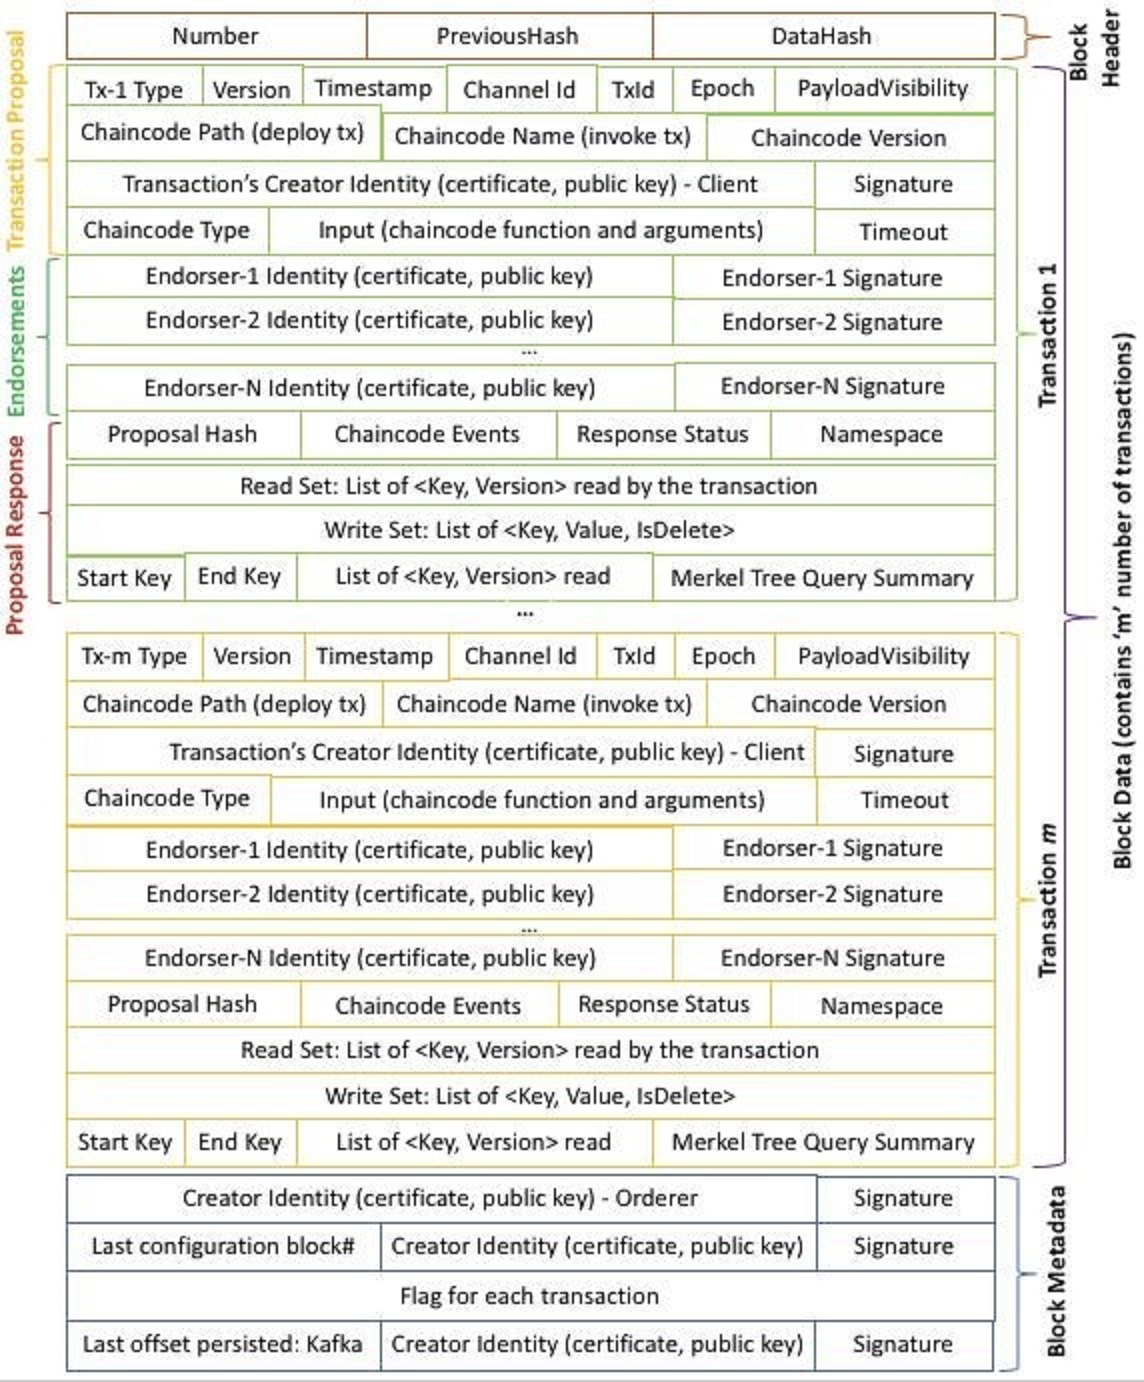
\includegraphics [scale=0.5] {hlf_block_structure}
	\caption{Структура блока Hyperledger Fabric}
	\label{fig:hlf_block_structure}
\end{figure}
\fi
\section{Типичные архитектуры Fabric ориентированных приложений} \label{sec:ch2:sec1}
Приложения взаимодействуют с сетью Hyperledger Fabric посредством SDK по протоколу gRPC как показано на рисунке \ref{fig:apps_use_sdk}. 
Они обращаются к узлам бизнес сети для вызова и/или запроса чейнкода, чтения данных из блокчейна, регистрируют слушателей событий, а так же выполня.т различные административные задачи такие как, запрос и/или изменение конфигурации узлов.
\begin{figure}[ht]
	\centering
	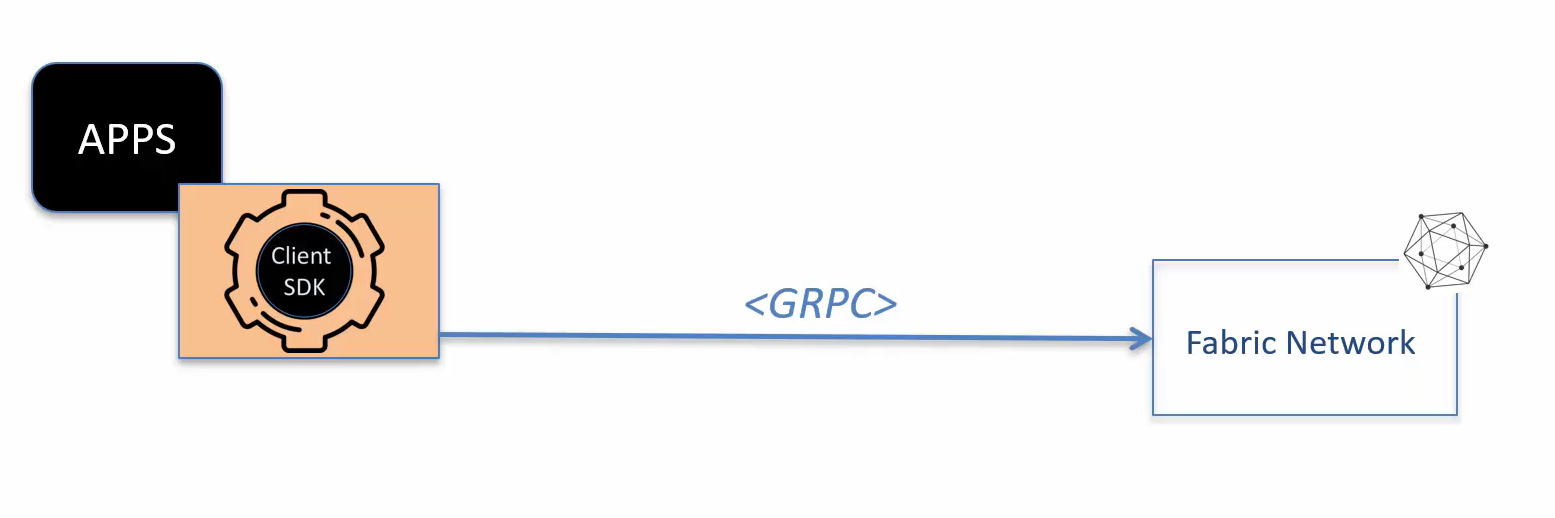
\includegraphics [scale=0.5] {apps_use_sdk}
	\caption{Взаимодействие приложений с Fabric Network}
	\label{fig:apps_use_sdk}
\end{figure}
Как уже упоминалось выше все эти операции осуществляются с помощью Fabric SDK для языков общего назначения. В настоящее время существуют Fabric SDK для языков Java, Go, Python и JavaScript. Так как каждую технологию следует выбирать для тех целей, для которых она подходит лучше всего, то будет справедливым рассмотреть типы Fabric ориентированных приложений. Чаще всего это:
\begin{itemize} 
	\item Графические приложения, позволяющие пользователю выполнять смарт-контракты через графический интерфейс.
	\item Приложения, представляющие отчеты из хранилища данных чейнкода.
	\item Модули интеграции Fabric SDK в уже существующие проекты, для взаимодействия с системами бекенда.
\end{itemize}
При разработки приложения того или иного типа уместно применение соответствующего шаблона архитектуры.
Рассмотрим типичные шаблоны построение Fabric ориентированных приложений.
Настольные приложения - создание и подписание транзакции посходит локально на компьютере пользователя. Такой подход является хорошо защищенным, но имеет недостаток в виде дистрибуции приложения. При внесении правок в приложение, конечный пользователь вынужден в ручную устанавливать обновления на свой компьютер.
\begin{figure}[ht]
	\centering
	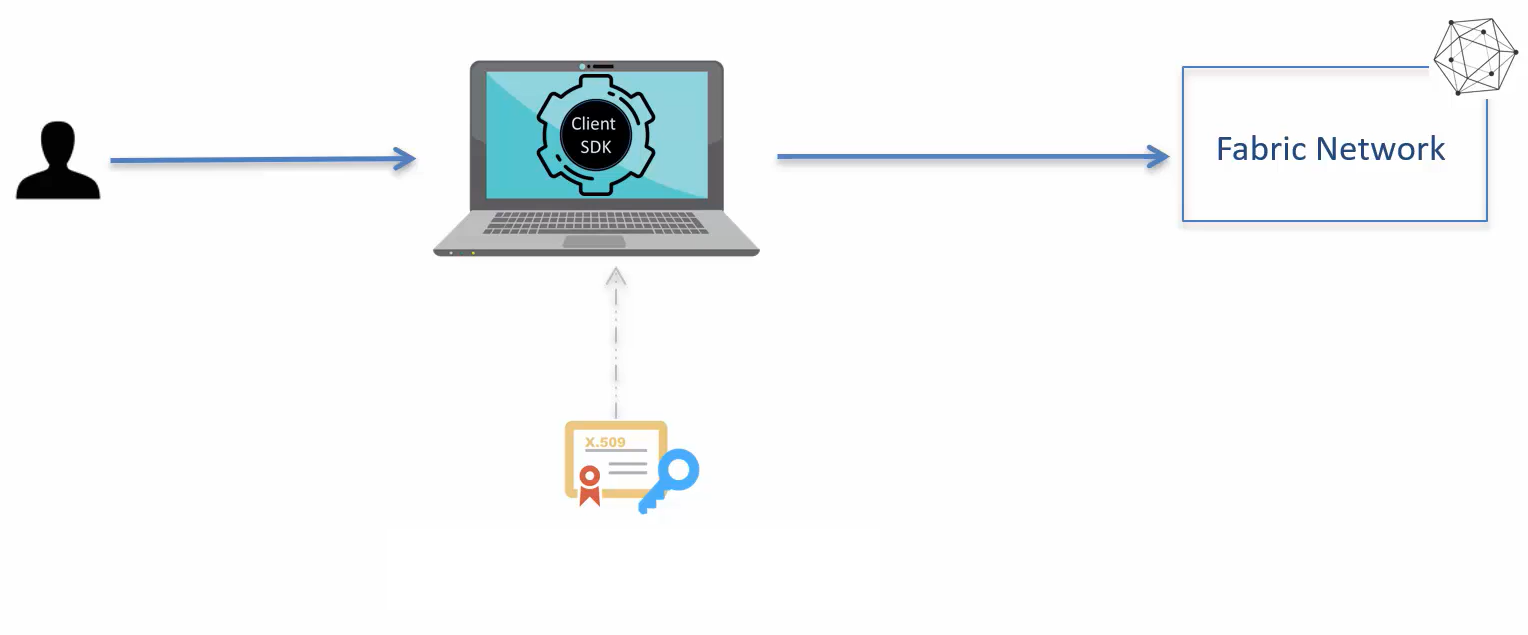
\includegraphics [scale=0.5] {desktop_apps}
	\caption{Настольные приложения, использующие Fabric SDK}
	\label{fig:desktop_apps}
\end{figure}
Обработка транзакций в сети Fabric приводит к возникновению различных событий, которые могут потребляется приложениями. События могут предоставятся клиента посредством некого брокера сообщений (например, Kafka), или же посредством REST-API. При получении определенного события клиентское приложение соответствующим образом обрабатывает его(например, обновляет свои бекенд системы). Так как события инициируются и обрабатываются в режиме реального времени, такой подход широко используется для создания инфопанелей и отчетов в режиме реального времени. Схематично данный шаблон предоставлен на рисунке 
\begin{figure}[ht]
	\centering
	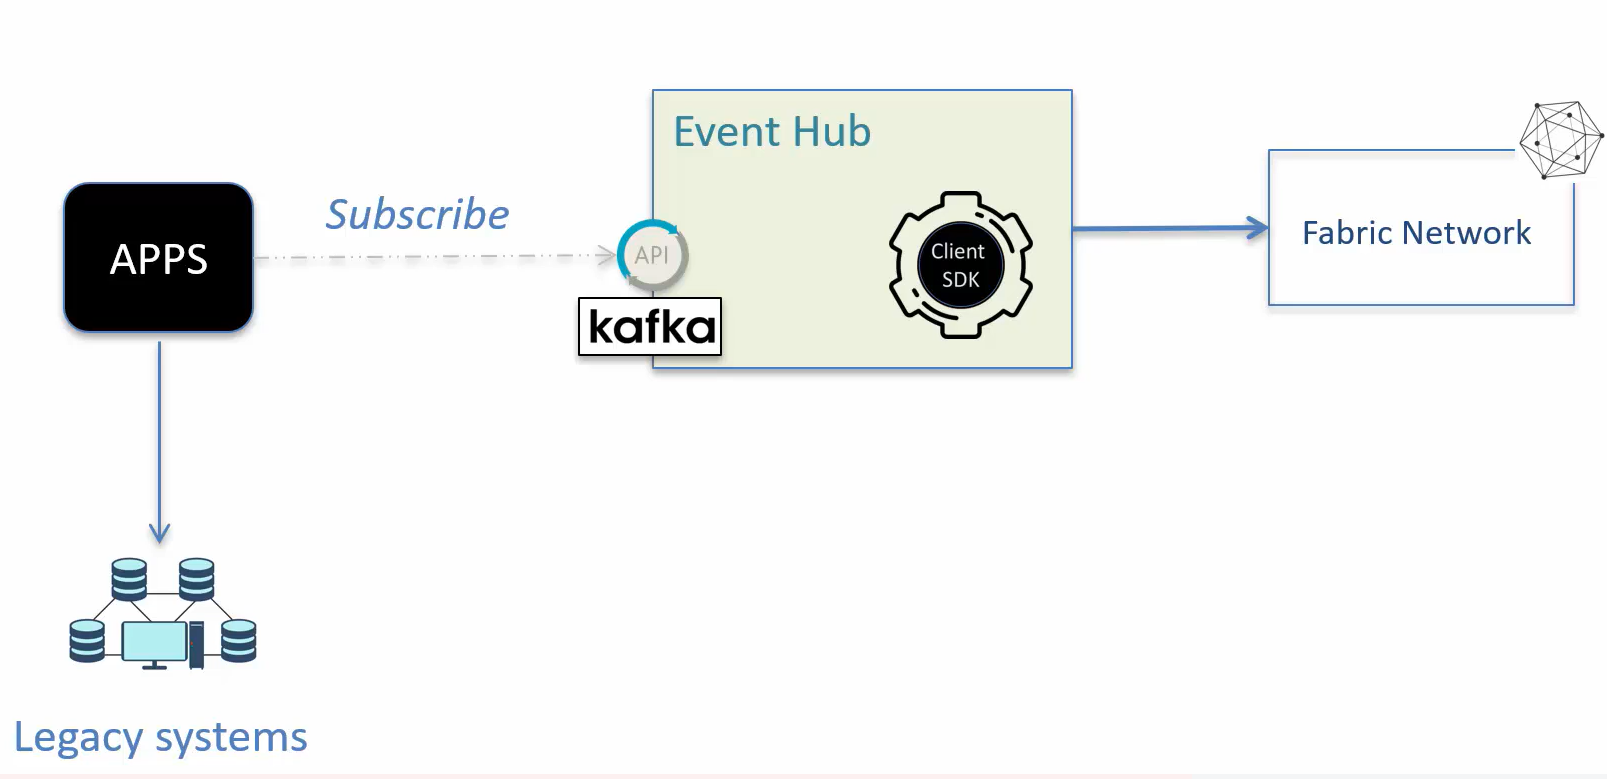
\includegraphics [scale=0.5] {event_hub}
	\caption{Архитектура "Event Hub"}
	\label{fig:event_hub}
\end{figure}
А также Fabric SDK может быть использована для создания различных утилит командной строки. Эти утилиты используется администраторами бизнес сети Hyperledger Fabric для осуществления различных административных задач (Рисунок \ref{fig:admin_cli}).
\begin{figure}[ht]
	\centering
	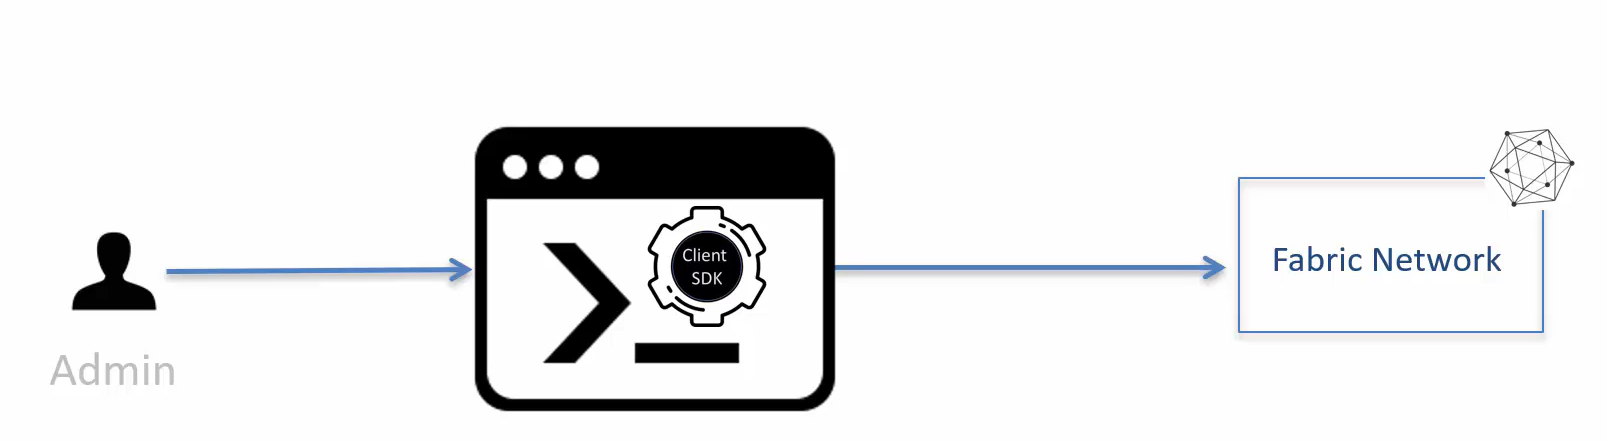
\includegraphics [scale=0.5] {admin_cli}
	\caption{Утилиты командной строки}
	\label{fig:admin_cli}
\end{figure}
Ещё один широк распространенный подход к построению Fabric ориентированных приложений - использование связующего программного обеспечения, ориентированное на обработку сообщений (англ. message-oriented middleware). Это ПО использует Fabric SDK, и обеспечивает связь среды выполнения Fabric с клиентским приложением. Middleware предоставляет API, обращаясь к которому клиентские приложения взаимодействуют с бизнес сетью. При этом тип клиентского приложения может быть любым(настольное, мобильное, веб и д.р.). Cхема такой архитектуры представлена на рисунке
\begin{figure}[ht]
	\centering
	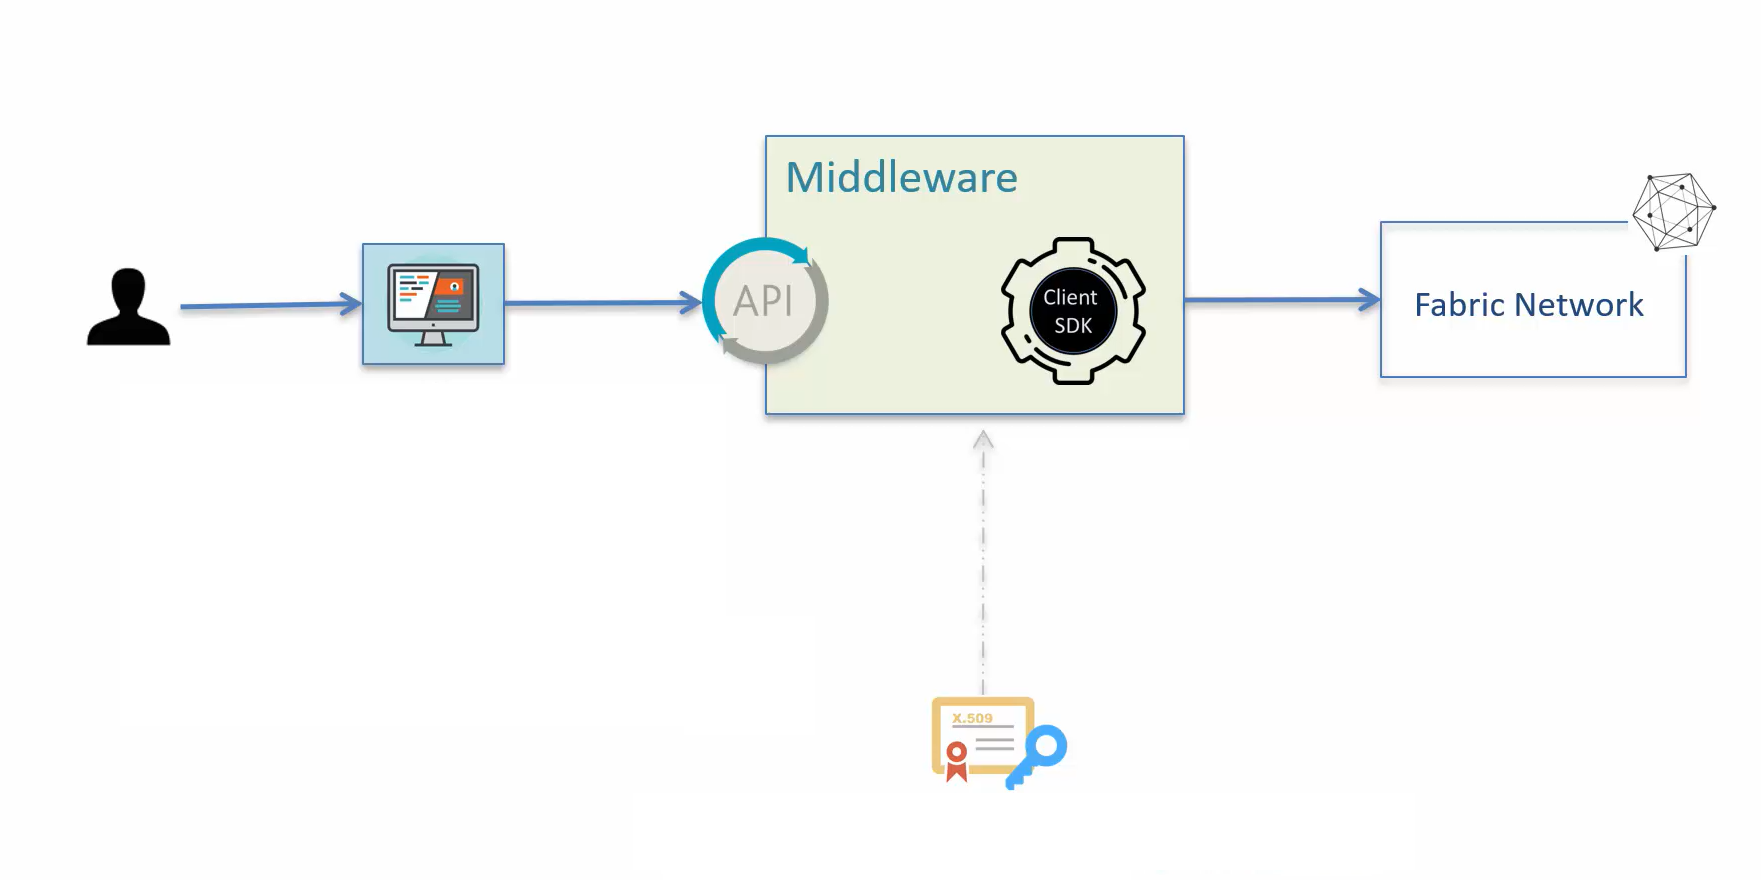
\includegraphics [scale=0.5] {middleware}
	\caption{Архитектура со связующим ПО}
	\label{fig:middleware}
\end{figure}
Но при реализации такого подход возникает ряд вопросов, и первый из них где управлять ключами и сертификатами пользователей? Один из вариантов - управлять ими на стороне middleware. Однако в этом случае пользователи должны доверять хосту middleware, т.к. их приватные ключи оседают на его стороне. Однако в некоторых случаях пользователи могут не доверять организации, осуществляющей хостинг middleware. В таких случаях необходимо закладывать логику работы с приватными ключами и сертификатами на стороне клиентского приложения. Очевидно, что такой подход является более защищенным, однако он так же имеет недостаток в виде увлечения сложности приложения. А также в этом случае нарушается принцип единственной ответственности (SRP). \cite{solid}


	%\section{Обеспечение безопасности REST-сервера} %\label{sec:ch2:sec2}
	%Как миниммум юзать TLS/HTTPs и аутентификацию.

\section{Выбор инструментов и технологий} \label{sec:ch2:sec2}
\subsection{Архитектура} \label{subsec:ch2/sec2/subsec1}
В \ref{sec:ch2:sec1} мы рассмотрели типичные архитектуры  Fabric ориентированных приложений. В данной работе выбор пал на архитектуру со связующим ПО с инкапсуляцией логики работы сертификатами пользователей на стороне связующего ПО. В представленных в работе сценариях отношение между отдельными элементами доверительные, поэтому недостаток данного подхода не создает проблем. К очевидными плюсам данной архитектуры можно, также отнести легкую замену графического клиентского приложения, т.к. ему неизвестно существование бизнес сети, оно работает исключительно со связующим ПО по технологии RPC. \cite{grpc}
На рисунке \ref{fig:sys_architecture} представлена схема архитектуры разработанного приложения.
\begin{figure}[ht]
	\centering
	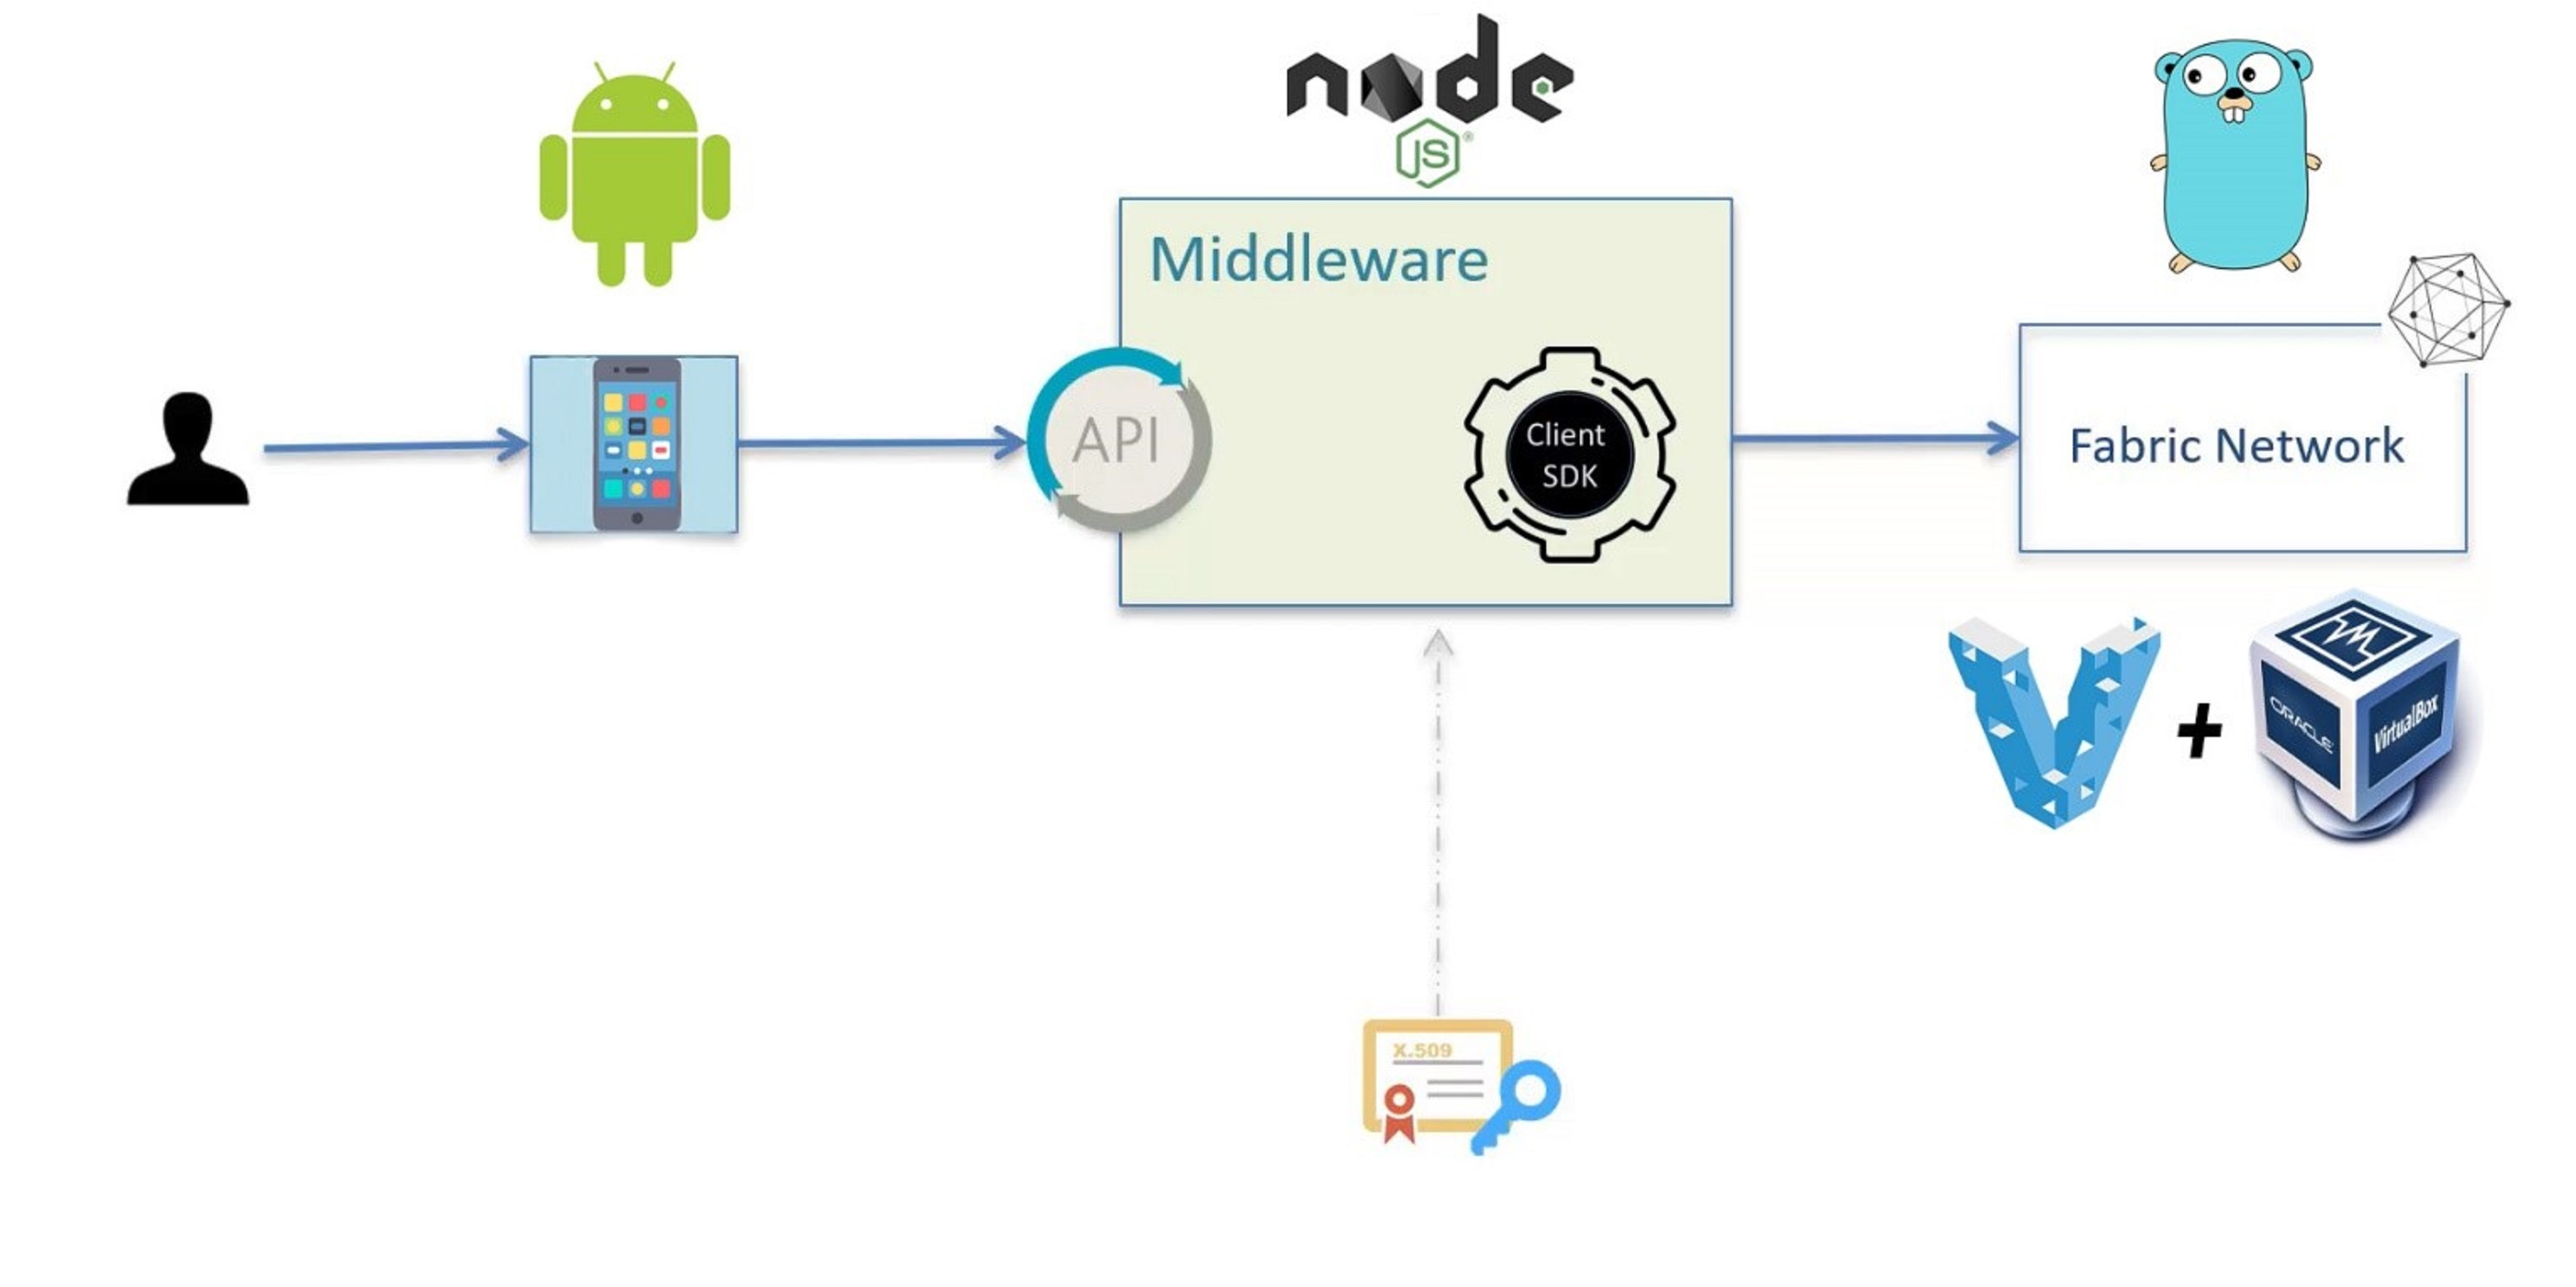
\includegraphics [scale=0.5] {sys_architecture}
	\caption{Архитектура разработанного приложения.}
	\label{fig:sys_architecture}
\end{figure}

\subsection{Смарт контракты} \label{subsec:ch2/sec2/subsec2}

 Есть СДК на нескольких языках, у нас на языке Go почему? ПОТОМУЧТО
 
\subsection{REST-сервер} \label{subsec:ch2/sec2/subsec3}
Для обеспечения связи клиентского приложение со связующим ПО в качестве методологии RPC был выбран REST (Representational State Transfer — передача состояния представления)\cite{restful} Философия этого подхода заключается в том, что приложения моделируются как набор ресурсов, с которыми клиенты могут взаимодействовать (считывать данные, обновлять, удалять и т.д.). В наше время построение приложений с помощью архитектурного стиля REST вкупе с HTTP и JSON\cite{js-json} стало фактическим стандартом для создания микросервисов.
Как уже упоминалось в \ref{sec:ch2:sec1}, Fabric SDK существует для нескольких языков программирования общего назначения, среди которых присутствует JavaScript \cite{pure-js}. 
TODO: Node js\cite{node-js}, npm, express

\subsection{Клиентское приложение}
 \label{subsec:ch2/sec2/subsec3}
 
Т.К. мобильное приложение, а самый распространенная система Андроид то конечно же джава
\iffalse
	Современные приложения редко работают в изоляции. Большинство из них общаются друг с другом по сети и координируют свои действия, обмениваясь сообщениями. Таким образом, современная программная система представляет собой набор распределенных приложений, которые работают на разных участках сети и взаимодействуют с помощью различных коммуникационных протоколов. Например, интернет-магазин может состоять из нескольких распределенных компонентов, таких как система управления заказами, каталог, база данных и т. д. Для реализации бизнес-возможностей подобного интернет-магазина необходимо наладить связь между этими компонентам.
	
	С появлением микросервисной и облачно-ориентированной архитектур традиционные приложения, обладающие разными бизнес-возможностями, подверглись разделению на более мелкие, автономные и бизнес-ориентированные сущности, известные как микро- сервисы. И эти микросервисы должны связываться друг с другом по сети, используя методики межпроцессного (межсервисного, межпрограммного) взаимодействия (inter-process communication, IPC). Существует несколько методик для осуществления межсервисного взаимодествия такие как SOAP, REST, RPC и другие. В данной работе выбор пал на методику REST, так как в наше время построение приложений с помощью архитектурного стиля REST вкупе с HTTP и JSON стало фактическим стандартом для создания микросервисов.  На рисунке \ref{fig:sys_architecture} показана архитектура разработанной системы, где Fabric Network и Middleware рассматриваются как отдельные микросервисы, взаимодействующие друг с другом. Все виды взаимодействий инициируются клиентом.
\fi
